\documentclass{article}
\usepackage{neb-macros}
\usepackage{tikz}
  \usetikzlibrary{calc}

\begin{document}

\CheapTitle{Plane Geometry}

\begin{dfn}[Plane Geometry]
Let $\mathcal{P}$ be an ordered geometry with a segment congruence and an angle congruence. We say that $\mathcal{P}$ is a \emph{plane geometry} if the following properties are satisfied.
\begin{itemize}
\item \textbf{Right Angle Property.} Any two right angles are congruent.

\item \textbf{Circle Separation.} If $o$, $a$, and $b$ are distinct points, then there is a unique point $c \in \Circle{o}{a} \cap \Ray{o}{b}$.

\begin{center}
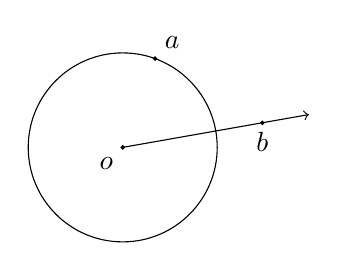
\begin{tikzpicture}[scale=0.6]
  \coordinate [label=below left:$o$]  (o) at (0  : 0);
  \draw [fill] (o) circle [radius=1pt];
  \coordinate [label=above right:$a$] (a) at (70 : 2);
  \draw [fill] (a) circle [radius=1pt];
  \coordinate [label=below:$b$]       (b) at (10 : 3);
  \draw [fill] (b) circle [radius=1pt];

  \draw [->] (o) -- (10: 4);
  \draw (o) circle [radius=2];
\end{tikzpicture}
\end{center}

\item \textbf{Circle Cut.} Let $o$, $a$, $p$, and $x$ be points, and suppose there are distinct points $u$ and $v$ on $\Circle{p}{x}$ such that $u \in \IntCircle{o}{a}$ and $v \in \ExtCircle{o}{a}$. Then $\Circle{o}{a} \cap \Circle{p}{x}$ contains two distinct points.

\begin{center}
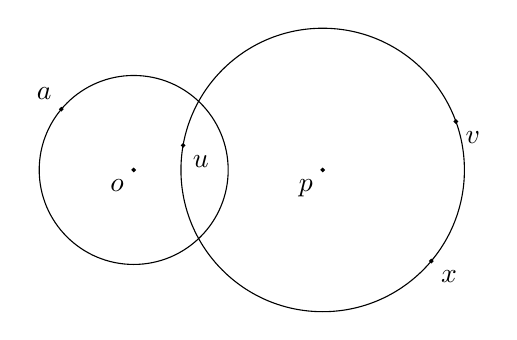
\begin{tikzpicture}[scale=0.6]
  \coordinate [label=below left:$o$]  (o) at (0,0);
  \draw [fill] (o) circle [radius=1pt];
  \coordinate [label=above left:$a$] (a) at ($ (o)+(140 : 2) $);
  \draw [fill] (a) circle [radius=1pt];
  \draw (o) circle [radius=2];

  \coordinate [label=below left:$p$]  (p) at (4,0);
  \draw [fill] (p) circle [radius=1pt];
  \coordinate [label=below right:$x$] (x) at ($ (p)+(320 : 3) $);
  \draw [fill] (x) circle [radius=1pt];
  \coordinate [label=below right:$u$] (u) at ($ (p)+(170 : 3) $);
  \draw [fill] (u) circle [radius=1pt];
  \coordinate [label=below right:$v$] (v) at ($ (p)+(20  : 3) $);
  \draw [fill] (v) circle [radius=1pt];
  \draw (p) circle [radius=3];


\end{tikzpicture}
\end{center}

\item \textbf{Circle Cut Transfer.} Suppose $a$, $b$, $c$, $d$, $x$, $y$, $z$, and $w$ are points such that $\Segment{a}{b} \equiv \Segment{x}{y}$, $\Segment{b}{c} \equiv \Segment{y}{z}$, and $\Segment{c}{d} \equiv \Segment{z}{w}$. If $\Circle{b}{a} \cap \Circle{c}{d}$ is not empty, then $\Circle{y}{x} \cap \Circle{z}{w}$ is not empty.

\item \textbf{Angle-Side Congruence.} Suppose $a$, $b$, $c$, $x$, $y$, and $z$ are points such that $\Segment{b}{a} \equiv \Segment{y}{x}$ and $\Segment{b}{c} \equiv \Segment{y}{z}$. Then $\Segment{a}{c} \equiv \Segment{x}{z}$ if and only if $\Angle{a}{b}{c} \equiv \Angle{x}{y}{z}$.
\end{itemize}
\end{dfn}

The Circle Separation and Circle Cut properties allow us to construct points on the intersection of a circle with a central ray and of two circles, respectively. (Without these we have no way to construct points on circles!) The Circle Cut Transfer property says that our geometry is ``uniform'' in some sense, allowing us to shift points in the intersection of two circles. Angle-Side Congruence provides an essential link between segment congruence and angle congruence, which are otherwise unrelated.

\subsection*{Some Consequences}

In the remainder of this section, suppose $\mathcal{P}$ is a plane geometry.

\begin{prop}[Circle Trichotomy]
Let $o$ and $a$ be distinct points. Then $\Circle{o}{a}$, $\IntCircle{o}{a}$, and $\ExtCircle{o}{a}$ partition the set of points in $\mathcal{P}$. That is, every point is either on $\Circle{o}{a}$, interior to $\Circle{o}{a}$, or exterior to $\Circle{o}{a}$.
\end{prop}

\begin{prop}[SSS Theorem]
If two triangles can be labeled such that corresponding sides are congruent, then the triangles are congruent. More precisely, let $a$, $b$, and $c$ be distinct points and $x$, $y$, and $z$ be distinct points. If $\Segment{a}{b} \equiv \Segment{x}{y}$, $\Segment{b}{c} \equiv \Segment{y}{z}$, and $\Segment{c}{a} \equiv \Segment{z}{x}$, then $\Triangle{a}{b}{c} \equiv \Triangle{x}{y}{z}$.
\end{prop}

\begin{proof}
That $\Angle{a}{b}{c} \equiv \Angle{x}{y}{z}$, $\Angle{b}{c}{a} \equiv \Angle{y}{z}{x}$, and $\Angle{z}{x}{y} \equiv \Angle{c}{a}{b}$ follows from three applications of the Angle-Side Congruence property.
\end{proof}

\begin{prop}[Uniqueness of Circle Cuts]
Let $o$, $a$, $p$, $x$, and $h$ be points, with $o$ and $p$ distinct and with $h$ not on $\Line{o}{p}$. There is at most one point $u \in \Circle{o}{a} \cap \Circle{p}{x}$ on the $h$-side of $\Line{o}{p}$.
\end{prop}

\begin{proof}
Suppose we have two such points, $u$ and $v$. That is, both $u$ and $v$ are on the $h$-side of $\Line{o}{p}$ and $u,v \in \Circle{o}{a} \cap \Circle{p}{x}$. Note that $\Segment{o}{p} \equiv \Segment{o}{p}$, $\Segment{p}{u} \equiv \Segment{p}{x} \equiv \Segment{p}{v}$, and $\Segment{u}{o} \equiv \Segment{a}{o} \equiv \Segment{v}{o}$. By the SSS Theorem, we have $\Triangle{u}{o}{p} \equiv \Triangle{v}{o}{p}$. In particular, we have $\Angle{u}{o}{p} \equiv \Angle{v}{o}{p}$ and $\Angle{u}{p}{o} \equiv \Angle{v}{p}{o}$. Now by AC7, we have $v \in \Ray{o}{u} \subseteq \Line{o}{u}$ and $u \in \Ray{p}{v} \subseteq \Line{p}{v}$. That is, $u$ and $v$ are points in the intersection of the lines $\Line{o}{u}$ and $\Line{p}{v}$. Since $o$ and $p$ are distinct, these lines must be distinct, and so they intersect at a unique point. Hence $u = v$.
\end{proof}

\begin{prop}[SAS Theorem]
If two triangles can be labeled such that two corresponding sides, and the angles between, are congruent, then the triangles are congruent. More precisely, let $a$, $b$, and $c$ be distinct points, and $x$, $y$, and $z$ be distinct points. If $\Segment{a}{b} \equiv \Segment{x}{y}$, $\Segment{b}{c} \equiv \Segment{y}{z}$, and $\Angle{a}{b}{c} \equiv \Angle{x}{y}{z}$, then $\Triangle{a}{b}{c} \equiv \Triangle{x}{y}{z}$.
\end{prop}

\begin{prop}[Pons Asinorum (Bridge of Asses)]
If $\Triangle{a}{b}{c}$ is isoceles with $\Segment{a}{b} \equiv \Segment{b}{c}$, then $\Angle{b}{a}{c} \equiv \Angle{b}{c}{a}$.
\end{prop}

\begin{proof}
We have two triangles, $\Triangle{b}{a}{c}$ and $\Triangle{b}{c}{a}$, such that $\Segment{b}{c}\equiv \Segment{b}{a}$, $\Segment{b}{a} \equiv \Segment{b}{c}$, and $\Angle{c}{b}{a} \equiv \Segment{a}{b}{c}$. By the SAS Theorem, $\Triangle{b}{a}{c} \equiv \Segment{b}{c}{a}$, and thus $\Angle{b}{a}{c} \equiv \Angle{b}{c}{a}$.
\end{proof}

\begin{cor}
Every triangle which is equilateral is also equiangular; all three interior angles are congruent.
\end{cor}

\begin{construct}[equilateral triangle with a given side]
Given distinct points $x$ and $y$, there exist points $z_1$ and $z_2$, on opposite sides of $\Line{x}{y}$, such that $\Triangle{x}{y}{z_1}$ and $\Triangle{x}{y}{z_2}$ are equilateral. In fact, we have $\Triangle{x}{y}{z_1} \equiv \Triangle{x}{y}{z_2}$.
\end{construct}

\begin{proof}
Consider the line $\Line{x}{y}$. By the Interpolation property, there exists a point $u$ such that $\Between{u}{x}{y}$. By the Circle Separation property, there is a point $w \in \Circle{y}{x} \cap \Ray{x}{w}$. Note in particular that $\Between{w}{x}{y}$, and hence $w$ is exterior to the circle $\Circle{y}{x}$. Moreover, $w$ is on $\Circle{x}{y}$. Now $y$ is also on $\Circle{x}{y}$, and by definition, $y$ is interior to $\Circle{y}{x}$. By the Circle Cut property, there exist two points in $\Circle{x}{y} \cap \Circle{y}{x}$, say $z_1$ and $z_2$, which must be on opposite sides of $\Line{x}{y}$ by the uniqueness of circle cuts. Now $\Segment{x}{z_1} \equiv \Segment{x}{y} \equiv \Segment{y}{z_1}$ and $\Segment{x}{z_2} \equiv \Segment{x}{y} \equiv \Segment{y}{z_2}$ by the definition of circles, so that $\Triangle{x}{y}{z_1}$ and $\Triangle{x}{y}{z_2}$ are equilateral by definition. Moreover, $\Triangle{x}{y}{z_1} \equiv \Triangle{x}{y}{z_2}$ by the transitivity of segment congruence and the SSS Theorem.
\end{proof}

\begin{prop}
Suppose $\Between{a}{b}{c}$ and $\Between{x}{y}{z}$. If any two of $\Segment{a}{b} \equiv \Segment{x}{y}$, $\Segment{b}{c} \equiv \Segment{y}{z}$, and $\Segment{a}{c} \equiv \Segment{x}{z}$ hold, then so does the third.
\end{prop}

\begin{proof}
Note that $\Angle{a}{b}{c} \equiv \Angle{x}{y}{z}$, $\Angle{b}{c}{a} \equiv \Angle{y}{z}{x}$, and $\Angle{c}{a}{b} \equiv \Angle{z}{x}{y}$ by AC4. The result then follows from the SAS Theorem.
\end{proof}

\begin{lem}
Suppose $\Between{a}{b}{c}$ and $y \in \Ray{x}{z}$. If $\Segment{a}{b} \equiv \Segment{x}{y}$ and $\Segment{a}{c} \equiv \Segment{x}{z}$, then $\Between{x}{y}{z}$.
\end{lem}

\begin{proof}
Since $y \in \Ray{x}{z}$, we have four possibilities: $y = x$, $\Between{x}{y}{z}$, $y = z$, and $\Between{x}{z}{y}$. If $y = x$, then we have $\Segment{a}{b} \equiv \Segment{x}{x}$, so that $b = a$, a contradiction. Similarly if $y = z$ then we have $\Segment{x}{y} \equiv \Segment{x}{z}$, so that $y = z$, also a contradiction. Now suppose that $\Between{x}{z}{y}$. Note that $\Angle{c}{a}{b} \equiv \Angle{z}{x}{y}$, $\Segment{a}{c} \equiv \Segment{x}{z}$, and $\Segment{a}{b} \equiv \Segment{x}{y}$; by the SAS Theorem, $\Triangle{a}{b}{c} \equiv \Triangle{x}{y}{z}$. In particular, the flat angle $\Angle{a}{c}{b}$ is congruent to the straight angle $\Angle{x}{z}{y}$, a contradiction. Thus $\Between{x}{y}{z}$ as claimed.
\end{proof}

\begin{construct}[copy a segment onto a ray]
Let $a$ and $b$ be distinct points, and let $o$ and $t$ be distinct points. There exists a point $x$ on $\Ray{o}{t}$ such that $\Segment{o}{x} \equiv \Segment{a}{b}$.
\end{construct}

\begin{proof}
First we construct a point $z$ such that $\Triangle{a}{o}{z}$ is equilateral; now $\Segment{z}{a} \equiv \Segment{z}{o}$. Using the Interpolation property, construct a point $h$ such that $\Between{z}{a}{h}$, and using the Circle Separation property, construct a point $u$ on $\Ray{a}{h}$ such that $\Segment{a}{u} \equiv \Segment{a}{b}$. Again using Circle Separation, construct a point $v$ on $\Ray{z}{o}$ such that $\Segment{z}{v} \equiv \Segment{z}{u}$. By the previous proposition, $\Between{z}{o}{v}$. Now $\Segment{z}{a} \equiv \Segment{z}{o}$ and $\Segment{z}{u} \equiv \Segment{z}{v}$, thus $\Segment{a}{u} \equiv \Segment{o}{v}$. Again using Circle Separation, construct a point $x$ on $\Ray{o}{t}$ such that $\Segment{o}{x} \equiv \Segment{o}{v}$. Then we have $\Segment{o}{x} \equiv \Segment{o}{v} \equiv \Segment{a}{u} \equiv \Segment{a}{b}$ as needed.
\end{proof}

\begin{construct}[copy an angle onto a ray]
Let $a$, $o$, $b$ be distinct noncollinear points and let $p$ and $x$ be distinct points. There exist two points $y_1$ and $y_2$, on opposite sides of $\Line{p}{x}$, such that $\Angle{x}{p}{y_1} \equiv \Angle{x}{p}{y_2} \equiv \Angle{a}{o}{b}$. 
\end{construct}

\begin{proof}
First copy segment $\Segment{o}{b}$ onto $\Ray{p}{x}$ at the point $u$, then copy the segment $\Segment{b}{a}$ onto the ray $\Ray{u}{p}$ at the point $v$. Now copy $\Segment{o}{a}$ onto $\Ray{p}{x}$ at the point $w$. Note that $\Segment{o}{a} \equiv \Segment{p}{w}$, $\Segment{o}{b} \equiv \Segment{p}{u}$, and $\Segment{b}{a} \equiv \Segment{u}{v}$. Moreover, the intersection $\Circle{o}{a} \cap \Circle{b}{a}$ is nonempty, as it contains $a$. By the Circle Cut Transfer property, $\Circle{p}{w} \cap \Circle{u}{v}$ contains two points $z_1$ and $z_2$ on opposite sides of $\Line{p}{x}$. By the SSS Theorem, we have $\Triangle{p}{u}{z_1} \equiv \Triangle{o}{b}{a} \equiv \Triangle{p}{u}{z_2}$, and thus $\Angle{u}{p}{z_1} \equiv \Angle{a}{o}{b} \equiv \Angle{u}{p}{z_2}$ as needed.
\end{proof}

\begin{prop}[ASA Theorem]
Let $a$, $b$, $c$ be distinct noncollinear points, and let $x$, $y$, $z$ be distinct points. If $\Angle{a}{b}{c} \equiv \Angle{x}{y}{z}$, $\Segment{b}{c} \equiv \Segment{y}{z}$, and $\Angle{b}{c}{a} \equiv \Angle{y}{z}{x}$, then $\Triangle{a}{b}{c} \equiv \Triangle{x}{y}{z}$.
\end{prop}

\begin{proof}
Copy $\Segment{y}{x}$ onto $\Ray{b}{a}$ at $d$. Note that $d$ and $a$ are on the same side of $\Line{b}{c}$. Moreover, we have $\Triangle{d}{b}{c} \equiv \Triangle{x}{y}{z}$ by the SAS Theorem, and so $\Angle{b}{c}{d} \equiv \Angle{y}{z}{x} \equiv \Angle{b}{c}{a}$. By AC7, we have $d \in \Ray{c}{a}$. Now $d$ is on both $\Line{b}{a}$ and $\Line{c}{a}$, and since $a$, $b$, and $c$ are not collinear, we must have $d = a$. So $\Triangle{a}{b}{c} \equiv \Triangle{x}{y}{z}$ as claimed.
\end{proof}

\end{document}
